\documentclass[a4paper]{article}

\usepackage[T1]{fontenc}
\usepackage[english]{babel}
\usepackage{graphicx}
\usepackage[nottoc]{tocbibind}
\usepackage[utf8]{inputenc}


%%%reqt stuff
\usepackage{hyperref}
\hypersetup{colorlinks=true, linkcolor=black, urlcolor=blue}
\usepackage[usenames,dvipsnames,svgnames,table]{xcolor}
\definecolor{entityColor}{RGB}{0,100,200}
\definecolor{attributeColor}{RGB}{0,100,50}
\definecolor{relationColor}{RGB}{160,0,30}
\usepackage{listings}
\lstdefinestyle{reqT}{
  belowcaptionskip=1\baselineskip,
  breaklines=true,
  showstringspaces=false,
  basicstyle=\footnotesize\sffamily,
  emph={Ent,Meta,Item,Label,Section,Term,Actor,App,Component,Domain,Module,Product,Release,Resource,Risk,Service,Stakeholder,System,User,Class,Data,Input,Member,Output,Relationship,Design,Screen,MockUp,Function,Interface,State,Event,Epic,Feature,Goal,Idea,Issue,Req,Ticket,WorkPackage,Breakpoint,Barrier,Quality,Target,Scenario,Task,Test,Story,UseCase,VariationPoint,Variant},
  emphstyle=\bfseries\color{entityColor},
  emph={[2]has,is,superOf,binds,deprecates,excludes,helps,hurts,impacts,implements,interactsWith,precedes,requires,relatesTo,verifies},
  emphstyle={[2]\bfseries\color{relationColor}},
  emph={[3]Attr,Code,Constraints,Comment,Deprecated,Example,Expectation,FileName,Gist,Image,Spec,Text,Title,Why,Benefit,Capacity,Cost,Damage,Frequency,Min,Max,Order,Prio,Probability,Profit,Value,Status},
  emphstyle={[3]\color{attributeColor}},  
}
\lstset{style=reqT}




%%%end reqt stuff




\title{System Requirements}
\author{Group D}
\date{\today}

\begin{document}
	\maketitle
	\thispagestyle{empty}
	\setcounter{page}{0}
	\pagebreak
	\tableofcontents
	\pagebreak
	
	% section background (end)

	\section{System Purpose} % (fold)
	The purpose of the system is to make everyday travels an easier task for people using public transportation. The users of this application will have an easily accessible overview over how long time it will take them to get to their favourite locations. These locations can be their work, home, the gym etc.
	\section{Domain}
		\begin{figure}[h]
				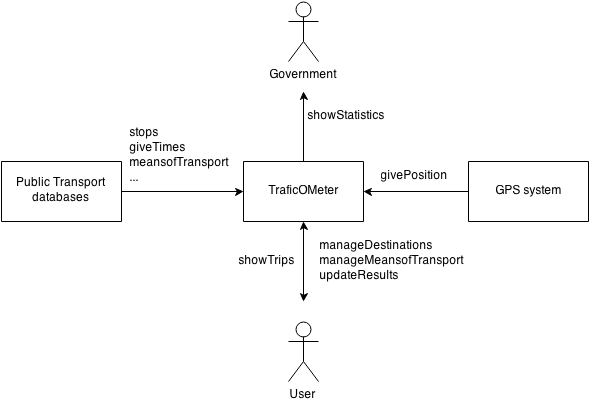
\includegraphics[scale=0.65]{Context-v1.png}
			\caption{Context Diagram for the system}
		\end{figure}
	\newpage
	\section{Data Requirements}
		The data in the data model should be stored by the system.	
		\begin{figure}[h]
			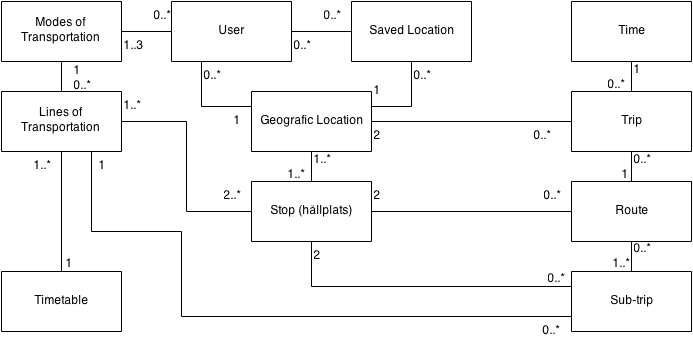
\includegraphics[scale=0.50]{datamodel-v1.png}
			\caption{Data Model for the system}
		\end{figure}	
	\section{Applications and Functional Requirements}
	\subsection{Tasks}
		

\begin{lstlisting}
Task addDestination
  Spec User saves a geographical location
Trigger: User want another destination to travel to
  Task Find Geographical Location
    Spec Locate a geographical location to travel to
    Variant Select current GPS-coordinates as geographical location
    Variant Desired geographical location does not exist
    Variant Multiple matches for geographical location query
    Frequency 5
  Task Name Geographical Location
    Spec Give a name to a geographical location
    Frequency 1
  Task Save Geographical Location
    Spec Save a geographical location to the device and database
    Frequency 1
  Why The user shall not have to search for a geographical location he/she might visit multiple times.
  Frequency 3
Task chooseTransportationMeans
  Spec User specifies which means of transportation(s) that the system shall use for calculating the fastest trip
  Frequency 1
Task removeDestination
  Spec Remove a previously added destination
  Task SelectDestination
    Spec Select a destination from a list of destinations
    Frequency 1
  Task deleteSelectedDestination
    Spec Remove a selected destination
    Frequency 1
  Frequency 1

\end{lstlisting}	
	\subsection{Feature Requirements}
	\begin{itemize}
			\item The System should support both Android and iOS units.
			\item The User should be able to search for destinations and save them.
			\item The User should be able to modify and remove saved destinations.
			\item The System should support multiple saved destinations.
			\item The System should be able to set the user's geografical position as a starting point.
			\item The System should support bus-, train- and ferry-travels in Sweden.
			\item The User should be able to specify which types of transportation it would like to use. 
			\item The System should automatically show the fastest travel option.
			\item The User should be able to select another travel option if the shown alternative does not fit its needs. This 				is preferrably done by swiping through different available alternatives.
			\item The User should be able to reach its saved destinations from different devices.
			\item The User should be able to see the time to reach it's saved destinations on the Mainscreen of the device.
		\end{itemize}
	\section{Operation Requirements}
	\section{Interface Requirements}
	\section{Quality Properties}
	\section{Documentation}
	
\end{document}
